\documentclass{tietreport}

% ==================================================
% PACKAGES
% ==================================================

\usepackage{graphicx}
\usepackage{float}
\usepackage{placeins}
\usepackage{array}
\usepackage{booktabs}

% Bibliography configuration
\usepackage[
  date=year,
  style=alphabetic,
  backend=biber,
  sorting=nty,
  maxnames=5,
  minnames=3,
  maxalphanames=4,
  minalphanames=3,
  backref=true,
  doi=false,
  isbn=false,
  url=false,
  eprint=false
]{biblatex}

\addbibresource{references.bib}

% All project images are stored in the images folder.
\graphicspath{{images/}}

% ==================================================
% PROJECT FIELDS
% ==================================================

\TitlePageHeader{%
  UCS503 - Software Engineering%
}

\ProjectTitle{%
  LedgerX%
}

\ProjectSubTitle{%
  A Decentralized Web3 Security Protocol for
  Protected Digital Asset Management and
  Real-Time Transaction Anomaly Detection%
}

% Replace the details below with your actual team details.
\author{%
  \texttt{1024030433} Ishan Rehan \\
  \texttt{1024030812} A S Danish \\
  \texttt{1024030813} Shreyansh Dua \\
  \texttt{1024030483} Shaurya Garg%
}

\TitlePageSubText{%
  Group: \texttt{3C55} BE Third Year, CSE%
}

\AdvisorName{%
  Dr. Nisha Thakur%
}

\TitlePageFooterText{{%
    \large Mid-Semester Evaluation \\[0.2cm]
    \bfseries Computer Science and Engineering
    Department%
  } \\[0.15cm]
  Thapar Institute of Engineering and Technology,
  Patiala%
}

% ==================================================

\begin{document}

\maketitle

\tableofcontents

% ==================================================
% CHAPTER 1: INTRODUCTION
% ==================================================

\chapter{Introduction}

\section{Background and Context}

The rapid growth of blockchain technology and decentralized
applications has resulted in an increasing number of users managing
cryptocurrency and other digital assets through blockchain-based
wallets and smart contracts. Blockchain provides transparency,
immutability, and decentralized control; however, these properties
alone do not guarantee protection against malicious transactions,
rug pulls, abnormal wallet activity, or other security threats.

Traditional cryptocurrency wallets primarily provide mechanisms for
storing, receiving, and transferring digital assets. The
responsibility of identifying suspicious transactions and responding
to potential threats is generally left to the user. This can create a
significant security risk because malicious transactions can occur
rapidly and may result in irreversible financial losses.

Smart contracts provide an opportunity to automate security
mechanisms directly on the blockchain. By encoding predefined rules
into smart contracts, a system can automatically perform
security-sensitive operations without depending entirely on manual
user intervention.

Machine learning can further improve this process by analysing
transaction characteristics and identifying behaviour that deviates
from normal transaction patterns. Combining blockchain-based
automation with anomaly detection therefore provides an opportunity
to create a more proactive approach to digital asset security.

LedgerX, also referred to as the SaveMe Protocol, is designed as a
decentralized Web3 security protocol that combines smart-contract
automation with transaction anomaly detection. The system provides a
protected wallet environment in which transactions can be monitored
and potentially suspicious activity can trigger an automated
protection mechanism.

The current web application provides users with an interface for
connecting a cryptocurrency wallet and accessing the major LedgerX
functions. These include sending assets, viewing transactions,
working with tokens, creating protocol-related assets, and viewing
the application's monitoring interface.

\subsection{Problem Statement}

Cryptocurrency users are exposed to several security threats,
including malicious transactions, abnormal wallet activity, and rug
pulls. Once a transaction has been executed on a blockchain, it is
generally difficult or impossible to reverse it through conventional
means.

Existing wallet systems primarily provide transaction functionality
but may require users to manually identify suspicious activity and
take appropriate action. This creates a gap between the detection of
a potential threat and the execution of a protective response.

The problem addressed by LedgerX is therefore the lack of an
integrated system that can monitor blockchain transactions, identify
potentially anomalous activity, and automatically initiate a
predefined protection mechanism to reduce the risk of digital asset
loss.

LedgerX addresses this problem by combining a protected
smart-contract-based wallet with transaction monitoring, anomaly
detection, liquidity conversion, and an automated asset-protection
workflow.

\section{Project Objectives}

The major objectives of LedgerX are:

\begin{enumerate}
  \item \textbf{Protected Wallet Creation:}
  Develop a smart-contract-based protected wallet that allows users
  to store and manage digital assets within an environment equipped
  with automated security mechanisms.

  \item \textbf{Transaction Anomaly Detection:}
  Implement a mechanism for analysing blockchain transactions and
  identifying potentially suspicious or abnormal activity.

  \item \textbf{Automated Threat Protection:}
  Develop an automated protection mechanism that can respond when
  suspicious activity is detected and initiate the appropriate
  security operations.

  \item \textbf{Liquidity Conversion and Fund Recovery:}
  Provide a mechanism for converting assets into a safer or more
  stable form and recovering protected funds for the asset owner
  when a threat is detected.

  \item \textbf{Transaction Monitoring:}
  Provide a user-friendly interface through which users can monitor
  wallet activity and inspect transaction history.
\end{enumerate}

These objectives are Specific because each objective corresponds to a
distinct capability of the LedgerX protocol. They are Measurable
through functional implementation and system-level evaluation. They
are Achievable using blockchain, smart-contract, web development,
and machine-learning technologies. They are Relevant to the problem
of improving digital-asset security and are Time-bound to the
development and evaluation milestones of the semester project.

% ==================================================
% CHAPTER 2: METHODOLOGY AND DESIGN
% ==================================================

\chapter{Methodology and Design}

\section{System Architecture}

LedgerX follows a modular architecture combining a web-based
frontend, blockchain smart contracts, transaction monitoring, and an
anomaly-detection component.

The frontend acts as the primary interaction layer through which
users connect their cryptocurrency wallets and interact with the
protocol. The blockchain layer contains the smart contracts
responsible for wallet management, asset transfers, liquidity
management, and security-related operations.

The anomaly-detection component analyses transaction characteristics
and identifies potentially suspicious activity. The result of this
analysis can be used to initiate the protection workflow.

The major components of the system are:

\begin{enumerate}
  \item \textbf{User Interface:}
  Provides the web-based interface for connecting wallets, sending
  assets, viewing transactions, working with tokens, and accessing
  the core LedgerX functionality.

  \item \textbf{Web3 Integration Layer:}
  Connects the frontend application to cryptocurrency wallets and
  deployed blockchain smart contracts.

  \item \textbf{Smart Contract Layer:}
  Implements protected-wallet functionality, asset management,
  liquidity operations, and automated protection mechanisms.

  \item \textbf{Anomaly Detection Layer:}
  Analyses transaction characteristics and identifies potentially
  abnormal or suspicious transactions.

  \item \textbf{Liquidity Layer:}
  Provides the mechanism required for converting assets into a safer
  form during the protection workflow.
\end{enumerate}

\subsection{High-Level Design}

The high-level design of LedgerX is represented through the
architectural and UML diagrams included in this chapter. The
diagrams describe the functional interactions, process flow,
component communication, data movement, and structural relationships
of the system.

\subsubsection{Use Case Diagram}

The Use Case Diagram identifies the main actors and the functions
available in the LedgerX system. The wallet owner interacts with the
system to connect a wallet, create a protected wallet, transfer
funds, monitor wallet activity, and view transaction information.
The security workflow includes anomaly detection, triggering the
self-destruct mechanism, token swapping, and returning protected
funds to the owner.

\begin{figure}[H]
    \centering
    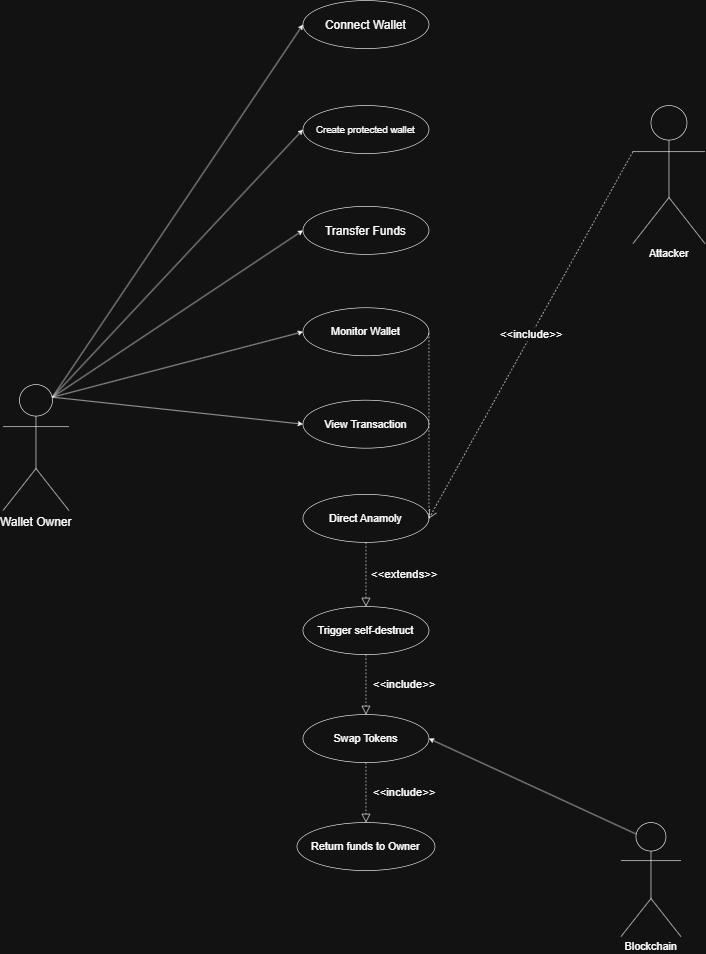
\includegraphics[width=0.78\textwidth]{use_case.png}
    \caption{Use Case Diagram of LedgerX}
    \label{fig:usecase}
\end{figure}

\FloatBarrier

\subsubsection{Activity Diagram}

The Activity Diagram represents the main workflow followed by a
LedgerX user. The process begins with wallet connection and protected
wallet creation, followed by transfer of funds and transaction
monitoring. If no threat is detected, monitoring continues. If a
threat is detected, the protection mechanism is triggered, assets
are swapped through the liquidity pool, and the recovered funds are
returned to the owner.

\begin{figure}[htbp]
    \centering
    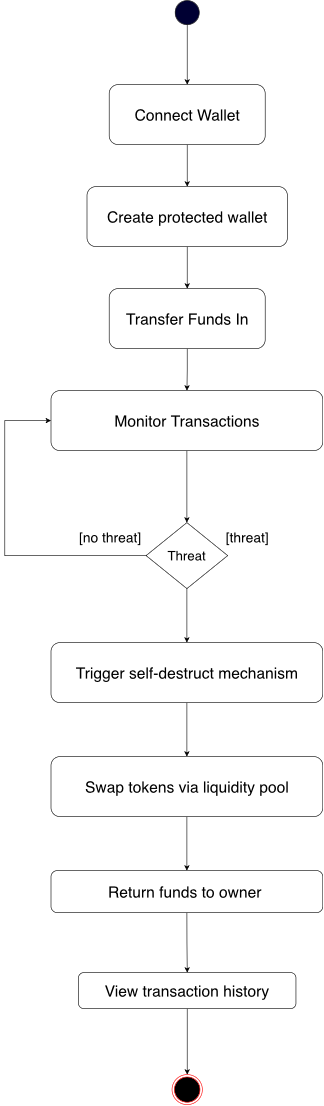
\includegraphics[width=0.27\textwidth]{activity_diagram.png}
    \caption{Activity Diagram of LedgerX}
    \label{fig:activity}
\end{figure}

\FloatBarrier

\subsubsection{Swimlane Activity Diagram}

The Swimlane Diagram provides another representation of the same
core workflow by separating responsibilities between the User,
System (Anomaly Guard), and Liquidity Pool. This representation
makes the responsibility of each subsystem explicit and shows how
control moves between the components during the protection process.

\begin{figure}[H]
    \centering
    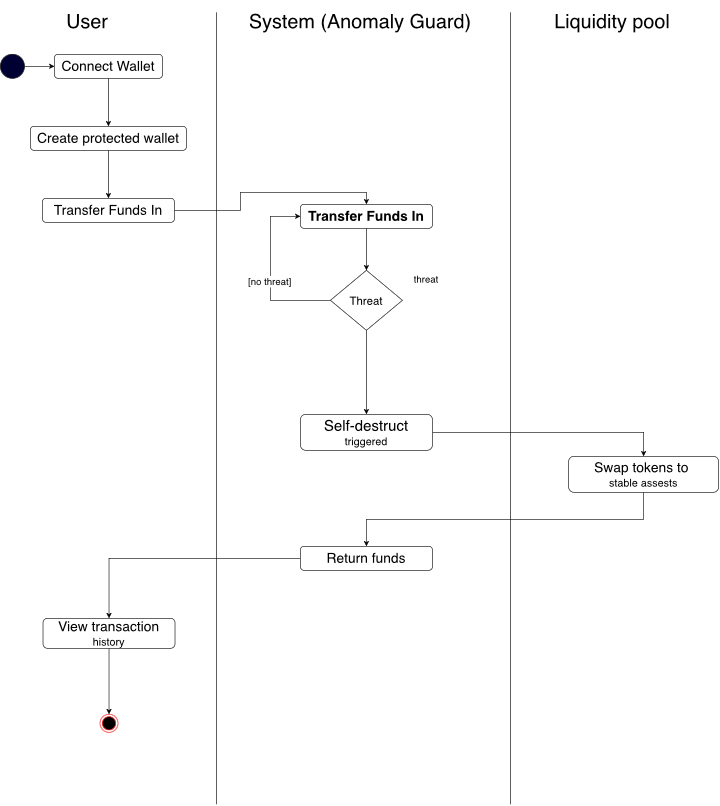
\includegraphics[width=0.68\textwidth]{swimlane_diagram.png}
    \caption{Swimlane Activity Diagram of LedgerX}
    \label{fig:swimlane}
\end{figure}

\FloatBarrier

\subsubsection{Sequence Diagram}

The Sequence Diagram describes the chronological interaction between
the User, Protected Wallet, Anomaly Guard, and Liquidity Pool. It
shows wallet connection and creation, transfer of funds, transaction
monitoring, anomaly detection, activation of the protection
mechanism, asset swapping, and return of recovered funds.

\begin{figure}[H]
    \centering
    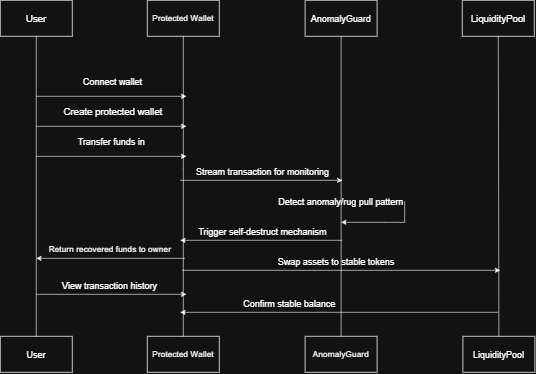
\includegraphics[width=0.90\textwidth]{sequence_diagram.png}
    \caption{Sequence Diagram of LedgerX}
    \label{fig:sequence}
\end{figure}

\FloatBarrier

\subsubsection{Data Flow Diagram}

The Data Flow Diagram represents how information moves through the
main functional stages of LedgerX. The user initiates wallet
management operations, transaction information is maintained as
transaction history, anomaly detection analyses the monitored
activity, and the swap and recovery process uses the resulting
security decision.

\begin{figure}[H]
    \centering
    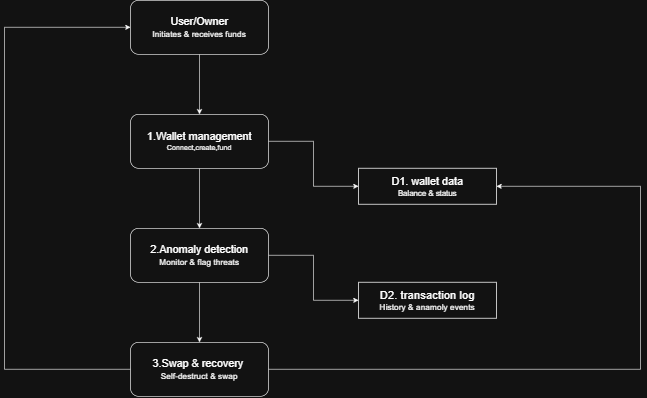
\includegraphics[width=0.88\textwidth]{dfd.png}
    \caption{Data Flow Diagram of LedgerX}
    \label{fig:dfd}
\end{figure}

\FloatBarrier

\subsubsection{Class Diagram}

The Class Diagram represents the structural relationships between the
main logical components of the LedgerX smart-contract system. The
diagram includes the Owner, Wallet, AnomalyGuard, and LiquidityPool
components and illustrates their responsibilities and relationships.

\begin{figure}[H]
    \centering
    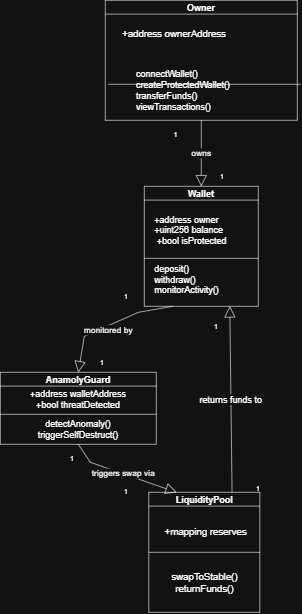
\includegraphics[width=0.52\textwidth]{class_diagram.png}
    \caption{Class Diagram of LedgerX}
    \label{fig:classdiagram}
\end{figure}

\FloatBarrier

\subsection{Technical Stack}

The LedgerX implementation combines web development, blockchain
technology, smart contracts, Web3 integration, and machine-learning
based anomaly detection.

\begin{itemize}
  \item \textbf{Frontend:}
  Next.js and React are used to implement the web-based user
  interface.

  \item \textbf{Programming Languages:}
  TypeScript/JavaScript are used for the web application and Solidity
  is used for blockchain smart contracts.

  \item \textbf{Blockchain and Smart Contracts:}
  Ethereum-compatible blockchain infrastructure is used for
  blockchain-based asset and security operations.

  \item \textbf{Smart Contract Development:}
  Hardhat and associated Ethereum development tools are used during
  smart-contract development.

  \item \textbf{Web3 Integration:}
  Web3 libraries are used to connect the frontend application with
  cryptocurrency wallets and blockchain contracts.

  \item \textbf{Machine Learning:}
  An Isolation Forest based approach is used for transaction anomaly
  detection.

  \item \textbf{Version Control:}
  Git and GitHub are used for source-code management and project
  collaboration.
\end{itemize}

\section{Implementation Details}

\subsection{Module 1: Core Functionality}

The core functionality of LedgerX is the combination of protected
wallet management, transaction monitoring, anomaly detection, and an
automated asset-protection mechanism.

The main workflow of the module is:

\begin{verbatim}
                    Connect Wallet
                         |
                         v
               Create Protected Wallet
                         |
                         v
                    Transfer Funds
                         |
                         v
                Monitor Transactions
                         |
                         v
                 Analyse Transaction
                         |
                  +------+------+
                  |             |
                Normal        Anomalous
                Activity       Activity
                  |             |
                  v             v
              Continue      Protection
              Monitoring     Mechanism
                                |
                                v
                          Convert Assets
                                |
                                v
                           Recover Funds
                                |
                                v
                         Return to Owner
\end{verbatim}

\subsubsection{Protected Wallet}

The protected wallet is the primary security component of LedgerX.
It provides an environment in which users can store and manage their
digital assets while enabling the protocol to monitor relevant
activity.

A user first connects a cryptocurrency wallet to the LedgerX
application. The user can then create a protected wallet through the
deployed smart-contract functionality. Assets can subsequently be
transferred into the protected environment.

\subsubsection{Transaction Monitoring}

LedgerX provides transaction monitoring functionality through its
web interface. The monitoring mechanism allows users to inspect
activities associated with the protected wallet.

Transaction information is important for the security layer because
the anomaly-detection component uses transaction characteristics to
determine whether the observed activity is consistent with expected
behaviour.

The monitoring functionality also improves transparency by allowing
users to inspect the history of operations performed within the
protocol.

\subsubsection{Anomaly Detection}

The anomaly-detection component is responsible for identifying
potentially suspicious transaction behaviour.

Transaction data is processed into relevant features that can be
provided to the machine-learning model. The model evaluates the
transaction and determines whether its behaviour is sufficiently
different from the expected transaction pattern to be classified as
an anomaly.

The general processing pipeline is:

\begin{verbatim}
                    Transaction Data
                           |
                           v
                    Feature Extraction
                           |
                           v
                    Data Preprocessing
                           |
                           v
                    Machine Learning Model
                           |
                           v
                    Anomaly Classification
                           |
                           v
                    Protection Decision
\end{verbatim}

The project uses an Isolation Forest-based approach for anomaly
detection. Isolation Forest is an unsupervised machine-learning
algorithm designed to identify observations that differ from the
majority of a dataset.

This approach is suitable for transaction monitoring because
malicious or abnormal transactions may exhibit characteristics that
differ significantly from normal transaction behaviour.

\subsubsection{Automated Protection Mechanism}

When suspicious activity is identified, LedgerX provides an
automated protection workflow. The purpose of this mechanism is to
reduce the time between detection of a potential threat and
execution of a protective action.

The protection mechanism is implemented through smart contracts so
that security-sensitive operations can be executed according to
predefined blockchain rules.

The protection workflow involves detecting abnormal activity,
initiating the protective mechanism, converting supported assets
through the liquidity mechanism, and recovering the protected funds
for the owner.

\subsubsection{Liquidity Conversion and Fund Recovery}

The protection workflow includes a liquidity conversion mechanism.
When the protection mechanism is activated, assets can be converted
into a safer or more stable form through the liquidity component.

The purpose of this step is to reduce exposure of the user's assets
during a potentially malicious event and provide a mechanism through
which protected funds can subsequently be recovered.

After the conversion process, the resulting assets are intended to be
returned to the designated owner through the smart-contract workflow.

\subsubsection{Frontend Implementation}

The current LedgerX frontend provides the primary user-facing
interface for interacting with the protocol. The landing page
introduces the protection concept and provides access to the wallet
connection functionality. The interface also exposes navigation for
sending assets, viewing transactions, managing tokens, creating
assets, and accessing the chart/monitoring functionality.

Figure~\ref{fig:frontendhome} shows the LedgerX landing page and
wallet-connection interface.

\begin{figure}[H]
    \centering
    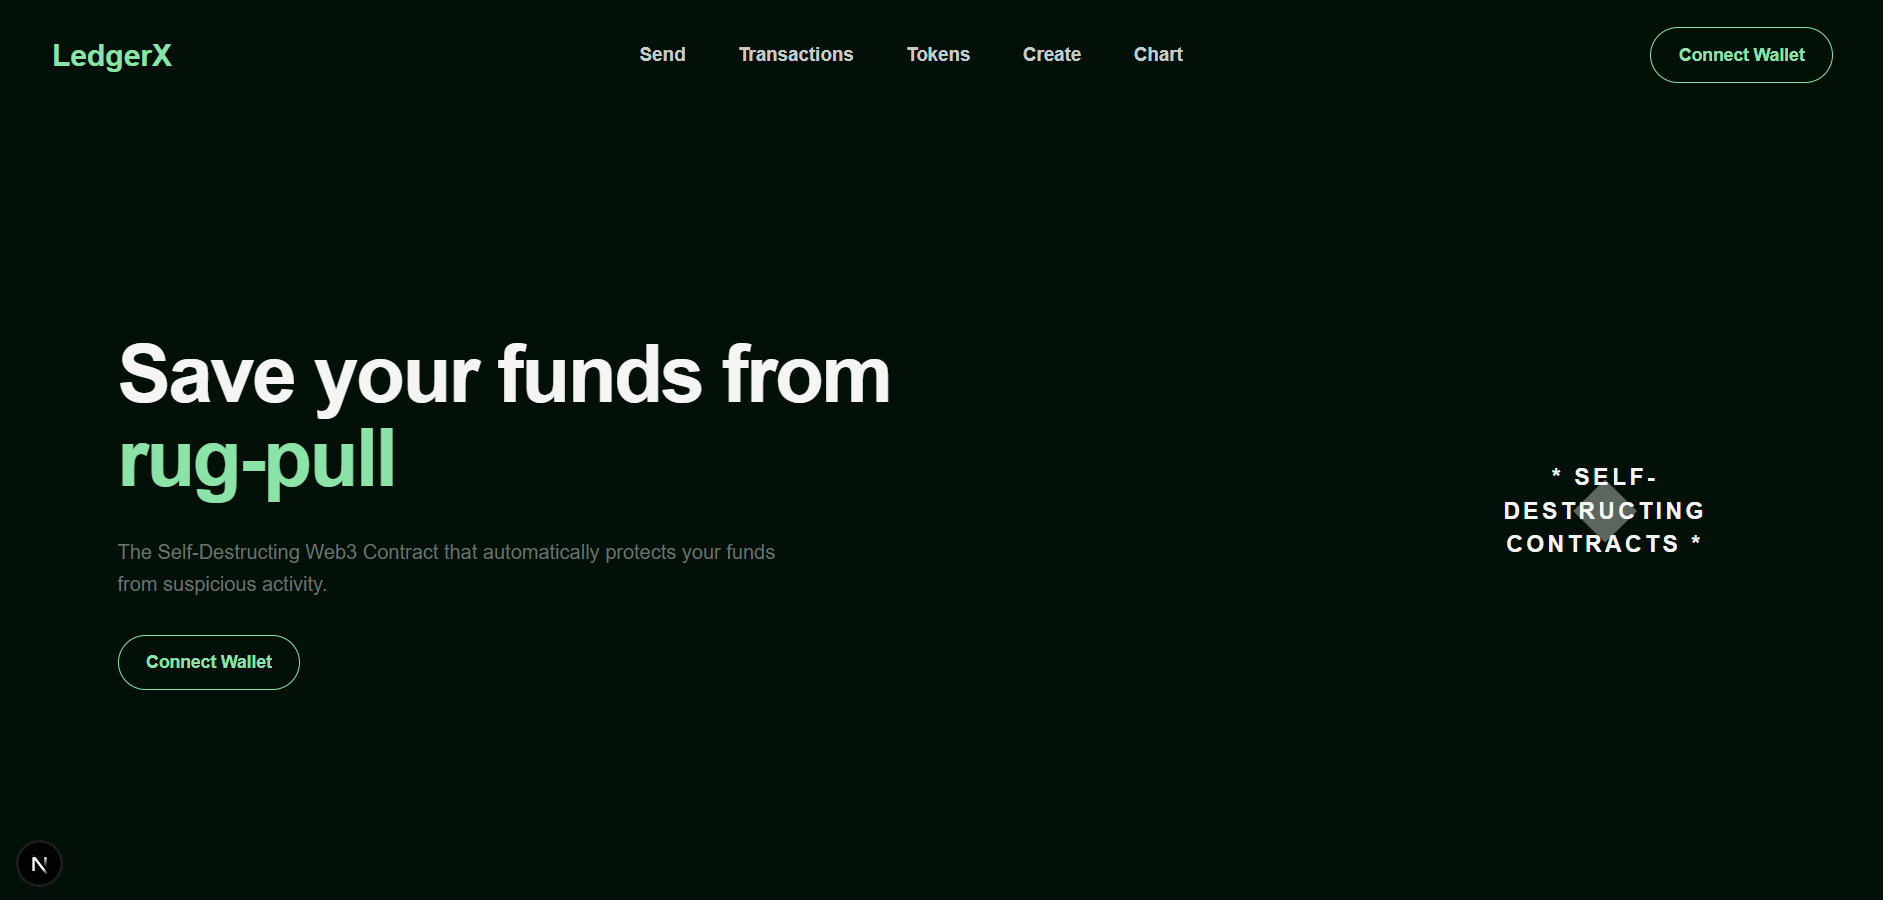
\includegraphics[width=\textwidth]{frontend_home.png}
    \caption{LedgerX Frontend Landing Page}
    \label{fig:frontendhome}
\end{figure}

\FloatBarrier

Figure~\ref{fig:frontendfeatures} shows the feature section of the
frontend, highlighting real-time anomaly detection, the
self-destruct mechanism, liquidity conversion, and fund recovery.

\begin{figure}[H]
    \centering
    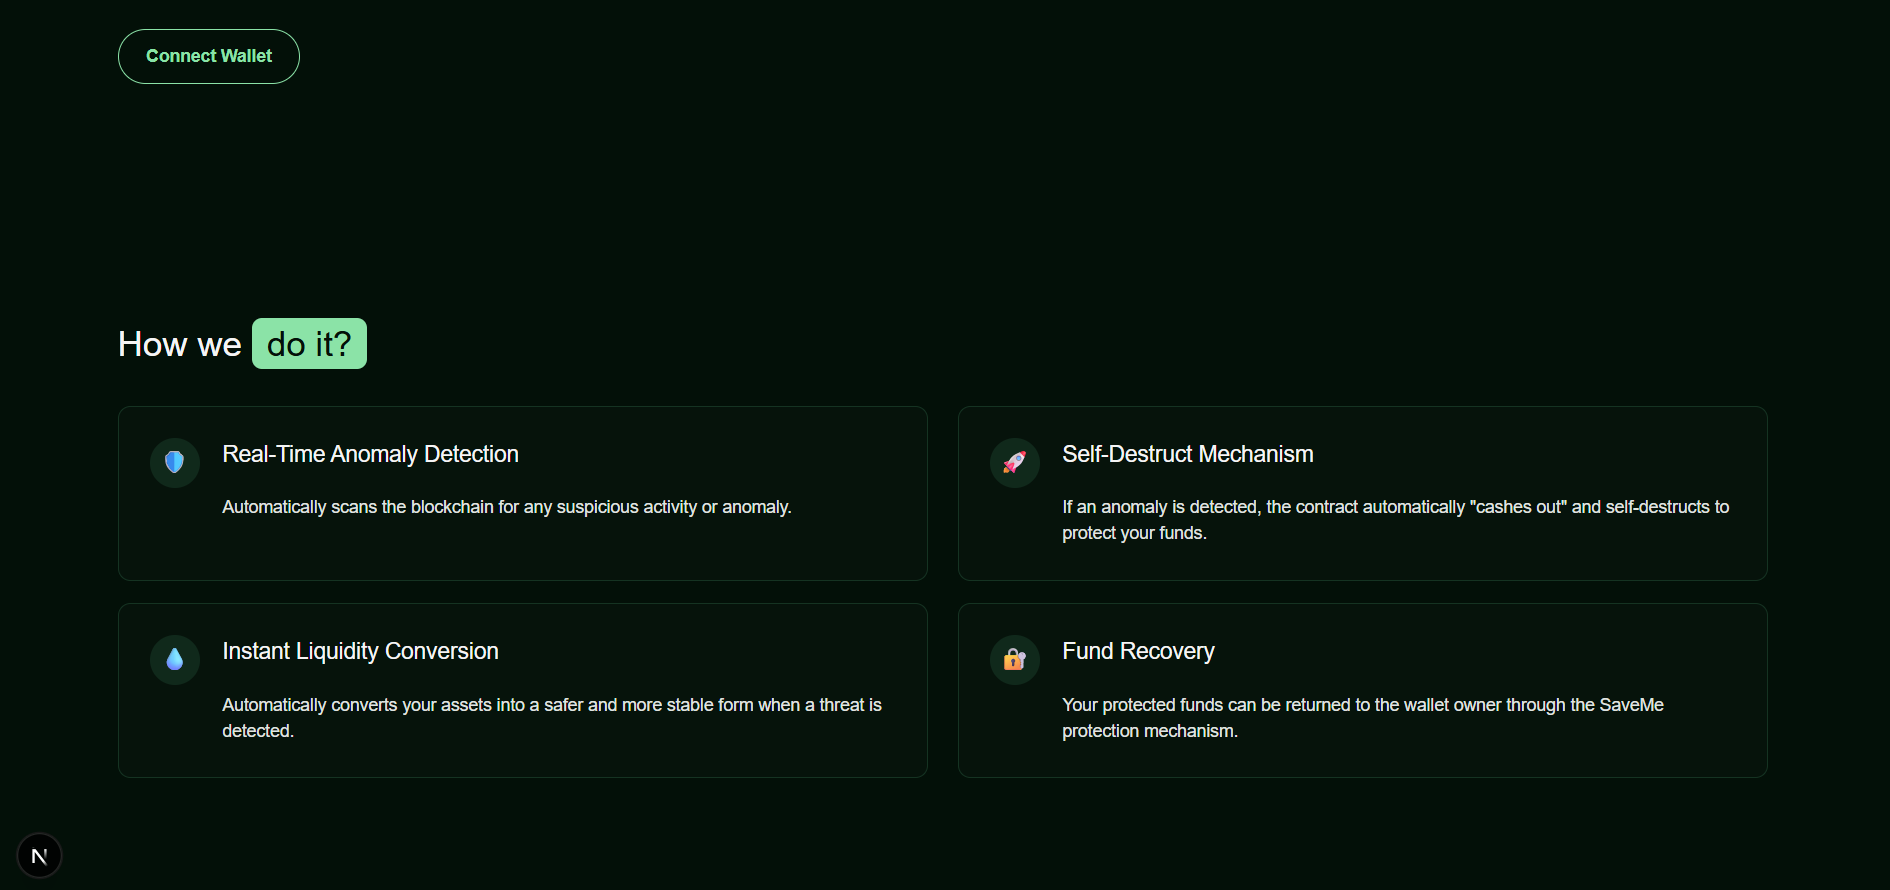
\includegraphics[width=\textwidth]{frontend_features.png}
    \caption{LedgerX Core Security Features}
    \label{fig:frontendfeatures}
\end{figure}

\FloatBarrier

The frontend screenshots demonstrate the current implemented user
interface and provide visual evidence of the core functionality
presented in this stage of the project.

\subsubsection{User Interaction Flow}

The complete user interaction with the core functionality can be
summarized as follows:

\begin{enumerate}
  \item The user opens the LedgerX web application.
  \item The user connects a supported cryptocurrency wallet.
  \item The user creates a protected wallet.
  \item The user transfers supported assets into the protected
  environment.
  \item Transactions associated with the wallet are monitored.
  \item Transaction characteristics are analysed by the anomaly
  detection component.
  \item If the transaction is considered normal, the transaction
  continues through the normal workflow.
  \item If potentially malicious activity is detected, the
  protection mechanism is activated.
  \item The protection mechanism can initiate asset conversion and
  fund recovery through the smart-contract and liquidity components.
  \item The protected funds are returned to the designated owner.
  \item The user can inspect the resulting transaction history.
\end{enumerate}

This completes the documentation of the core functionality included
in the current stage of LedgerX.

% ==================================================
% BIBLIOGRAPHY
% ==================================================

\printbibliography[heading=bibintoc]

\end{document}
